\section{Grundlagen}

\begin{description}
\item[Aufbau] \fbox{Applikation} -> \fbox{DBMS(Datenbank-Management-System)} -> \fbox{Datenbanken}
\item[Persistenz:] nicht-flüchtig gespeichert nach Transaktionsende
\item[Konsistenz:] Widerspruchsfrei, durch Integritätsregeln
\item[Redundanz:] Mehrfaches vorkommen von Daten => Lösen durch Normalisierung
\item[Isolation:] Keine Beieinflussung von Nutzern untereinander
\item[Semantische Integrität:] korrekt aus Fachsicht 
\item[Operationale Integrität:] konsistenz / Integrität während Systembetrieb erhalten
\item[ACID:] Atomicity, Consistency,Isolation,Durability; Gegenpart bei Verteilten: BASE
\item[Datenmodell:] definiert Operatoren und Objekte (relational, netzwerk,xml,...)
\item[Logisches Schema:] Struktur der Daten
\item[Physisches Schema:] Indizes etc,
\item[Entity Integrity:] eindeutigkeit der PKs
\item[Referentielle Integrität:] Datensätze erst löschen, wenn nicht mehr referenziert
\item[Domänen Integrität:] Werte atomar, liegen in Definierten Wertebereichen (CHECK)
\item[Surrogat-Schlüssel:] künstlicher Primärschlüssel (id)
\item[CAP-Theorem:] Konsistenz, Verfügbarkeit, Toleranz gegen Netzausfall: nur 2 von 3 möglich
\item[3Schichten-Modell:] \begin{minipage}{0.3\textwidth}
\begin{tabular}{|c|}
\hline
Externe Ebene(Views) \\\hline Logische Ebene(Schema) \\\hline Interne Ebene (Indizes)\\\hline
\end{tabular}\end{minipage}
\item[Physische Datenunabhänigkeit:] Anwendung unabhängig von Interner Ebene 
\item[Logische Datenunabhängigkeit:] Anwendung fast unabhängig von Logischer Ebene 
\end{description}


\section{Umsetzung von Vererbung}
\halfpage{
\begin{description}
\item [Single Table] alles in einer Tabelle, die Kind-Attribute sind ggf. NULL \\
Vorteile: Redundanzfrei, keine JOINs \\
Nachteile: Viel NULL, Große Tabelle, nicht über mehrere Ebenen
\item [Table-per-Class (Joined Subclass)]: jede Klasse eigene Tabelle \\
Vorteile: Redundanzfrei, Einfacher Zugriff auf typunabhängige Attribute der Oberklasse, keine NULL-Werte  \\
Nachteile: JOINs nötig => schlechtere Performance, Referentielle Integrität muss geprüft werden
\item  [Table-per-Concrete-Class (Leaf Model)]: nur Tabellen für Klassen mit Instanzen \\
Vorteile: Typen leicht unterscheidbar, Objektinformation in einer Tabelle \\
Nachteile: ggf. Redundante Informationen, Anfragen über alle Objeke: UNION
\end{description}
}

Kardinalitäten: 1:1, 1:n, n:m, + optionalität

Identifizierende Beziehungen: schwache Entität setzt andere Entität voraus (z.B. Bestellpositionen Bestellung)
\subsection*{Chen-Notation}
\usetikzlibrary{er}
\tikzset{multi attribute/.style={attribute,double distance=1.5pt}}
\tikzset{derived attribute/.style={attribute,dashed}}
\tikzset{total/.style={double distance=1.5pt}}

\newcommand{\key}[1]{\underline{#1}}

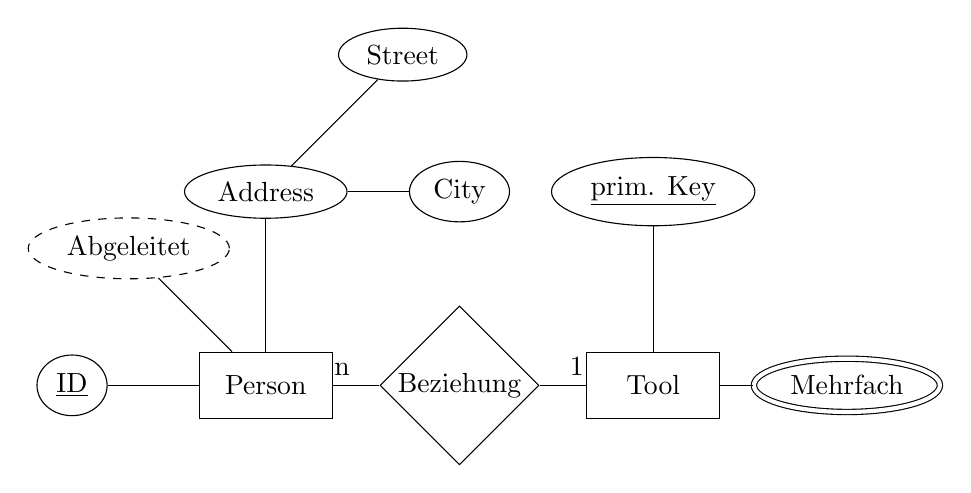
\begin{tikzpicture}[node distance=7em]
\node[entity](person){Person};
\node[attribute](pid)[left of=person]{\key{ID}}edge(person);
\node[attribute](address)[above of=person]{Address}edge(person);
\node[attribute](street)[above right of=address]{Street}edge(address);
\node[attribute](city)[right of=address]{City}edge(address);
\node[derived attribute](age)[above left of=person]{Abgeleitet}edge(person);
\node[relationship](uses)[right of=person]{Beziehung}edge(person);
\node[entity](tool)[right of=uses]{Tool}edge(uses);
\node[attribute](tid)[above of=tool]{\key{prim. Key}}edge(tool);
\node[multi attribute](phone)[right of=tool]{Mehrfach}edge(tool);
\draw(tool) -- (uses) node[pos=0.2,above] {1};
\draw(uses) -- (person) node[pos=0.8,above] {n};
\end{tikzpicture}

\def\pk#1{\node[name=\entityname-#1, every property/.try]{#1};\node[name=\entityname-#1, every property/.try, red, text width=1in, align=right]{(PK)};\\}
\def\fk#1{\node[name=\entityname-#1, every property/.try]{#1};\node[name=\entityname-#1, every property/.try, red, text width=1in, align=right]{(FK)};\\}


\subsection*{Krähenfuß}
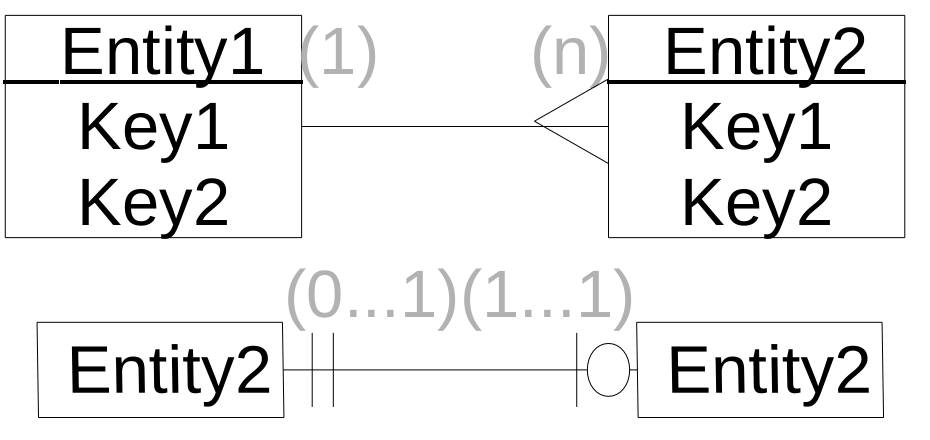
\includegraphics[width=0.2\textwidth]{crow}
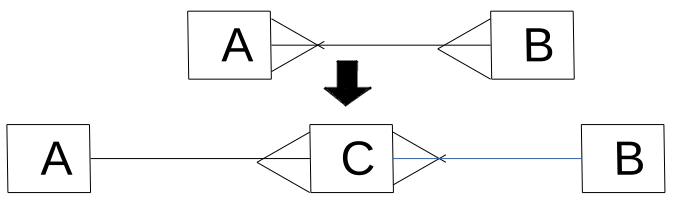
\includegraphics[width=0.2\textwidth]{m-n}


